% !TEX root = ../5.DISTILLATION.tex
\section{EXPERIMENTAL RESULTS}

\subsection{Raw Data}

\begin{table}[H]
    \centering
    \caption{Raw experimental results}
    \label{tab:raw_data}
    \small
    \begin{tabular}{ccccccccccc}
        \toprule
        \textbf{No} & \textbf{Loc.} & \textbf{F}       & \textbf{D}       & \textbf{Reflux} & \multicolumn{2}{c}{\textbf{Conc. (\%)}} & \multicolumn{4}{c}{\textbf{Temp. ($^\circ$C)}}                                                       \\
        \cmidrule(lr){6-7} \cmidrule(lr){8-11}
                    & \textbf{Feed} & \textbf{(ml/min)} & \textbf{(ml/min)} & \textbf{$L_o$}  & \textbf{Feed}                           & \textbf{Dist.}                                 & \textbf{$t_F$} & \textbf{$t_W$} & \textbf{$t_D$} & \textbf{$t_{Lo}$} \\
        \midrule
        1           & 4             & 150               & 44               & 7               & 10                                      & 45                                             & 57             & 93             & 38             & 88                \\
        2           & 4             & 150               & 59               & 10              & 10                                      & 55                                             & 58             & 96             & 38             & 83                \\
        3           & 4             & 150               & 28               & 15              & 10                                      & 45                                             & 58             & 93             & 38             & 79                \\
        4           & 2             & 150               & 36               & 10              & 10                                      & 50                                             & 55             & 96             & 37             & 78                \\
        5           & 5             & 150               & 46               & 10              & 10                                      & 50                                             & 64             & 96             & 38             & 77                \\
        \bottomrule
    \end{tabular}
\end{table}

\subsection{Data Processing}

\begin{table}[H]
    \centering
    \caption{Raw results processing (mol fractions)}
    \label{tab:processing}
    \begin{tabular}{cccccccc}
        \toprule
        \textbf{No} & \textbf{Loc.} & \textbf{F}\footnote{Calibration factor: $V_{ml/min} = V_{reading} \times 5.64$} & \textbf{D}       & \textbf{Reflux} & \textbf{$x_F$} & \textbf{$x_D$} & \textbf{$x_W$} \\
                    & \textbf{Feed} & \textbf{(ml/min)} & \textbf{(ml/min)} & \textbf{$L_o$}  &                &                &                \\
        \midrule
        1           & 4             & 150.0             & 44.0             & 39.48           & 0.0416         & 0.242          & 0.032          \\
        2           & 4             & 150.0             & 59.0             & 56.40           & 0.0416         & 0.323          & 0.016          \\
        3           & 4             & 150.0             & 28.0             & 84.60           & 0.0416         & 0.242          & 0.032          \\
        4           & 2             & 150.0             & 36.0             & 56.40           & 0.0416         & 0.281          & 0.016          \\
        5           & 5             & 150.0             & 46.0             & 56.40           & 0.0416         & 0.281          & 0.016          \\
        \bottomrule
    \end{tabular}
\end{table}

\begin{table}[H]
    \centering
    \caption{Calculation Results}
    \label{tab:calculations}
    \begin{tabular}{cccccccc}
        \toprule
        \textbf{No} & \textbf{Loc.} & \textbf{R} & \textbf{$t_F$} & \textbf{$H_F$} & \textbf{$H_{GF}$} & \textbf{$H_{LF}$} & \textbf{$q$} \\
        \midrule
        1           & 4             & 0.90       & 57             & 235            & 2983              & 308               & 1.065        \\
        2           & 4             & 0.96       & 58             & 238            & 2983              & 307               & 1.063        \\
        3           & 4             & 3.02       & 58             & 238            & 2963              & 287               & 1.063        \\
        4           & 2             & 1.57       & 55             & 225            & 3003              & 327               & 1.069        \\
        5           & 5             & 1.23       & 64             & 262            & 3005              & 330               & 1.052        \\
        \bottomrule
    \end{tabular}
\end{table}

\begin{table}[H]
    \centering
    \caption{Operating lines and efficiency results}
    \label{tab:lines}
    \begin{tabular}{cccccc}
        \toprule
        \textbf{No} & \textbf{Input line}  & \textbf{Rectification line} & \textbf{$n_{LT}$} & \textbf{Ratio\footnote{Likely $\frac{n_{LT}}{n_{actual}}$ as per original notes}} & \textbf{$E_o$} \\
        \midrule
        1           & $y = 16.38x - 0.64$  & $y = 0.47x + 0.13$          & 1                 & 0.2 & 0.20          \\
        2           & $y = 16.87x - 0.66$  & $y = 0.49x + 0.17$          & 2                 & 0.4 & 0.40          \\
        3           & $y = 16.87x - 0.66$  & $y = 0.75x + 0.06$          & 1                 & 0.2 & 0.20          \\
        4           & $y = 15.49x - 0.60$  & $y = 0.61x + 0.11$          & 2                 & 0.4 & 0.40          \\
        5           & $y = 20.23x - 0.80$  & $y = 0.55x + 0.13$          & 2                 & 0.4 & 0.40          \\
        \bottomrule
    \end{tabular}
\end{table}

\subsection{Graphical Analysis}

Schematic calculation of theoretical trays was performed for each experiment using the Python calculation suite. The resulting McCabe-Thiele diagrams are shown in Figure \ref{fig:mt_plots}.

\begin{figure}[H]
    \centering
    \begin{subfigure}[b]{0.45\textwidth}
        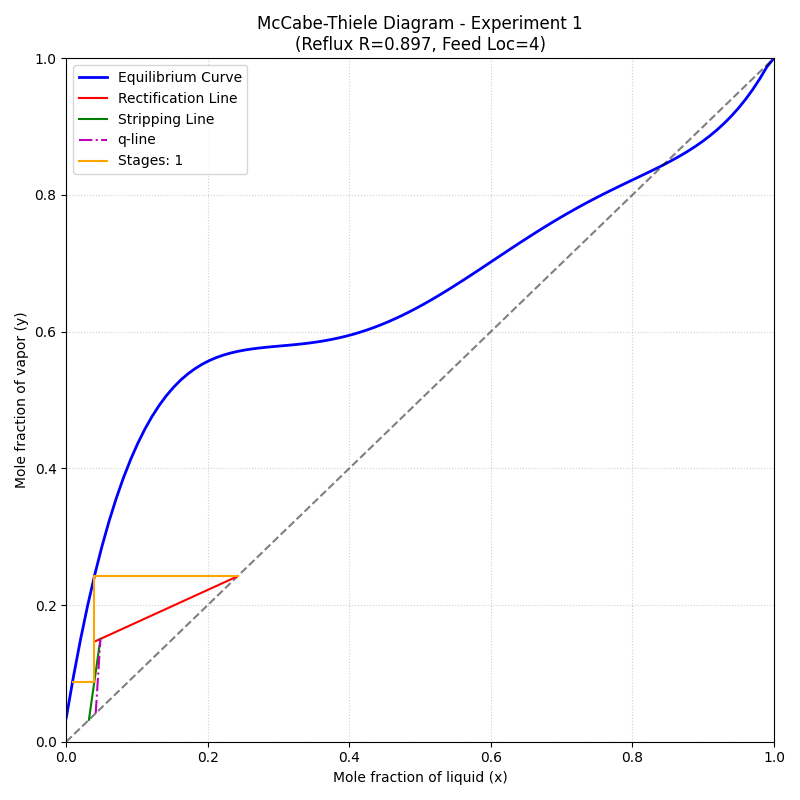
\includegraphics[width=\textwidth]{Figures/plot_1.png}
        \caption{Experiment 1}
    \end{subfigure}
    \hfill
    \begin{subfigure}[b]{0.45\textwidth}
        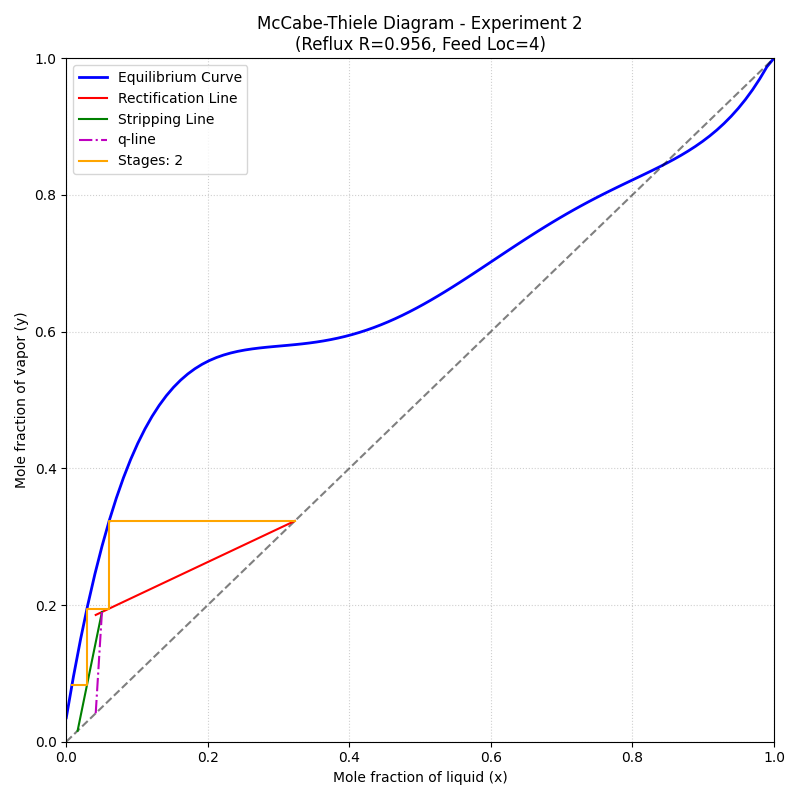
\includegraphics[width=\textwidth]{Figures/plot_2.png}
        \caption{Experiment 2}
    \end{subfigure}

    \vspace{0.5cm}

    \begin{subfigure}[b]{0.45\textwidth}
        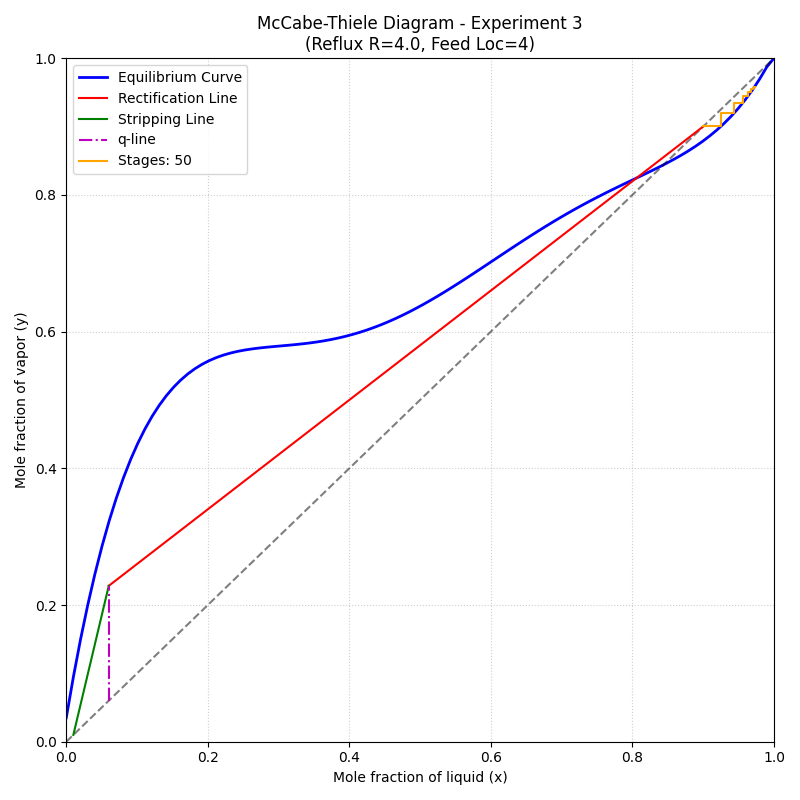
\includegraphics[width=\textwidth]{Figures/plot_3.png}
        \caption{Experiment 3}
    \end{subfigure}
    \hfill
    \begin{subfigure}[b]{0.45\textwidth}
        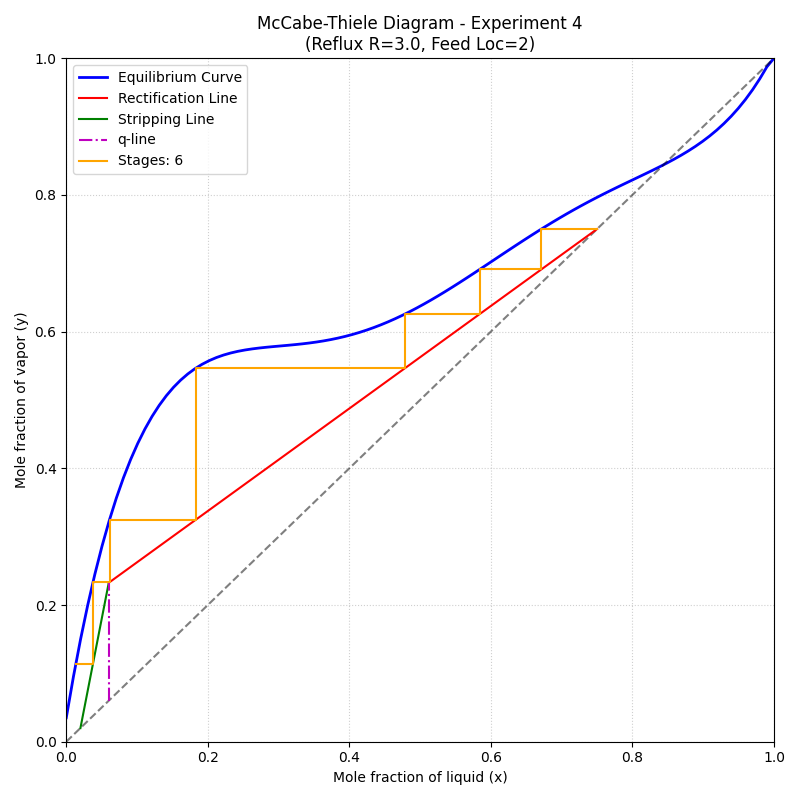
\includegraphics[width=\textwidth]{Figures/plot_4.png}
        \caption{Experiment 4}
    \end{subfigure}

    \vspace{0.5cm}

    \begin{subfigure}[b]{0.45\textwidth}
        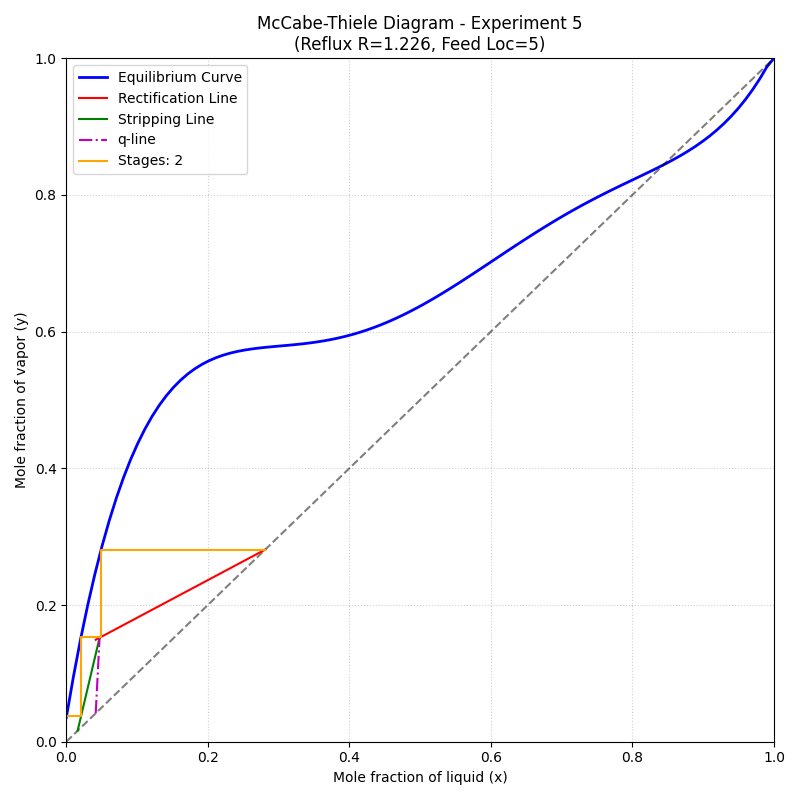
\includegraphics[width=\textwidth]{Figures/plot_5.png}
        \caption{Experiment 5}
    \end{subfigure}
    \caption{McCabe-Thiele diagrams for all five experiments.}
    \label{fig:mt_plots}
\end{figure}
